\section{Achieving superlinear scaling in the Linux kernel}\label{sec:case-study}

Next, we present a case study for systematically applying the distributed self-adjusting systems architecture to a common networking problem: software packet classification \cite{gupta2001algorithms}. The goal is to demonstrate the general engineering methodology by assembling \emph{existing} techniques into a distributed self-adjusting scheme and understand when, and to what extent, superlinear scaling emerges. We consider it a success if we can robustly reproduce faster-than-linear growth on some realistic workloads. It is a stated \emph{nongoal} to conceive novel algorithms, let alone produce the fastest software packet classifier. % (that award undeniably goes to DPDK \texttt{rte\_acl} \cite{rte-acl})
Yet, our self-adjusting firewall will prove several times faster than the default Linux kernel implementation on a wide range of workloads.

To achieve superlinear scaling we need a self-adjusting algorithm in the first place (plus a locality-boosting load balancer). From the many potential use cases % for which a self-adjusting algorithm exists
\cite{SleatorT85Splay, BentleyCL93, HesterH85, HesterH85, BentleySTW86, Avin0020, ParkM12} we eventually chose packet classification for the following reasons.  First, the default Linux firewall implementation, \nftables, uses a static doubly linked list to evaluate classifier rules, which makes it an appealing candidate for applying the move-to-front (MTF) heuristics (but see ramifications related to handling rule-dependencies below). % which will buy us the non-self-adjusting baseline for free.
Second, underlying packet classification there is an infamously difficult theoretical problem \cite{10.1145/2619239.2626294,10.1006/jagm.1996.0063, PacutVAPRS2022, 10.1145/2619239.2626294, 10.1145/1851182.1851208, 10.1145/863955.863980, gupta2001algorithms}, % , 10.1145/3359989.3365431},
and achieving superlinear speedup on such a hard problem promises massive performance gain. Third, the Linux kernel network stack offers several flexible software and hardware based load balancers for dispatching packets to parallel classifier instances running on different CPU cores \cite{rss-linux}, which we will reuse to implement the locality-boosting load balancer component. And fourth, packet classifiers are very difficult to cache \cite{1354643} (recall, caches are the ``cheap'' way to obtain superlinear scaling), which calls for a true self-adjusting packet classifier. % algorithm that goes beyond caching. % \cite{10228937}.

% \subsection{The Linux packet classifier}
% \label{sec:sa-pack-class}

\subsection{Self-adjusting packet classification}
\label{sec:sa-sa-pack-class}

A network firewall is a means to control incoming and outgoing network traffic based on user-defined packet classifier rules (see Fig.~\ref{fig:class-sample}). % This is useful to improve security, control access, filter and protect against ongoing attacks, and log\slash monitor network activity.
A classifier \emph{rule} is a pair of a filter, a user-defined regular expression defined on specific fields of the packet header or metadata, and an action that decides what to do with the packets that match the filter (accept, drop, log, etc.).  Rules are organized into linear chains ordered by rule priority. When a packet enters a chain, it is compared against the first rule. If there is a match, the corresponding action is executed and the lookup is over. Otherwise, subsequent rules are matched in priority order until the first match is found.

% The Linux kernel contains several built-in packet classifiers.
The \nftables kernel engine adds a virtual machine to the Linux kernel that uses a DSL for parsing and matching packet header fields \cite{nftables}. This makes \nftables agnostic to specific network protocols, in contrast to, e.g., \texttt{iptables}, which contains an embedded protocol parser. Currently, \nftables is the default packet classifier in most Linux distributions.

\begin{figure}[t]
  \centering
  \begin{small}
    \renewcommand{\tabcolsep}{2pt}
    \begin{tabular}{r|l|l|r|r|l}
      \textbf{Prio} & \textbf{Proto} & \textbf{Src IP} & \textbf{Dst IP} & \textbf{Dst Port} & \textbf{Action}\\
      \hline
      1 & UDP & 192.168.178.33   & 23.0.0.45  & 53  & ACCEPT\\
      2 & TCP & 10.10.10.0/24    & 23.0.0.45  & 443 & DROP\\
      3 & UDP & 192.168.178.0/24 & 23.0.0.45  & 53  & DROP\\
      4 & TCP & 10.10.10.10/32   & 23.0.0.45  & ANY & ACCEPT\\
      5 & IP  & 192.168.0.0/16   & 23.0.0.0/8 &     & ACCEPT\\
    \end{tabular}
  \end{small}%
  \caption{Sample firewall rule set. Source ports do not matter.}
  \label{fig:class-sample}
\end{figure}

One way to make \nftables self-adjusting would be to replace the static linked list it uses internally for rule matching with a self-adjusting list. A naive application of MTF, however, would easily break the semantics of the firewall. This is because rules in the chain may not be independent from each other, and hence may not be freely swapped \cite{10.1145/2619239.2626294}.

Consider the example in Fig.~\ref{fig:class-sample} and suppose that, initially, rules are ordered priority-wise in the list: $\langle1, 2, 3, 4, 5\rangle$. Suppose that a packet with the IP 5-tuple (192.168.0.1, 23.0.0.45, UDP, 1, 3478) enters the classifier, where the fields in the 5-tuple are IP source and destination address, protocol, and source and destination port, respectively. Rules are inspected in linear order until rule 5 is found as the first match, at which point the lookup terminates with the verdict ACCEPT. Now, a naive application of MTF would move rule 5 to the front of list, resulting in the order $\langle5, 1, 2, 3, 4\rangle$. Suppose another packet with the 5-tuple (192.168.178.1, 23.0.0.45, UDP, 1, 53) is to be processed next: this will immediately match rule 5 at the front of the list yielding the verdict ACCEPT, despite that, if matched in priority order, rule 3 would be the correct match and the verdict should be DROP. % To maintain correctness, the furthest we can move rule 5 towards the front of the list is the position immediately after its dependency, rule 3.

We say that rule $u$ is \emph{dependent} on another rule $v$ if they have overlapping match criteria in all fields, $v$ has a higher priority than $u$, and $u$ and $v$ define different actions. Such a dependency means that $u$ is not allowed to be moved before $v$ in the list, otherwise some packets may be erroneously classified. For instance, in the example of Table~\ref{fig:class-sample} rule 5 is dependent on rule 3, which is in turn dependent on rule 1, implying the dependency chain $5\to 3\to 1$. Similarly, rule $4$ is dependent on rule $2$. % Rule dependencies define a Directed Acyclic Graph (DAG) in the graph whose nodes are the set of rules, where there is an edge $(u, v)$ from $u$ to $v$ if $u$ is dependent on $v$ (see Fig.~\ref{fig:class-dep}).

% \begin{figure}[t]
%   \centering
%   \begin{small}
%     \begin{tikzpicture}[->,>=stealth,node distance=2.5cm, auto, every node/.style={circle,draw,minimum size=0.5cm,inner sep=2pt}]
%       % Branch 1
%       \node[circle,draw] (5) {5};
%       \node[circle,draw,right of=5] (3) {3};
%       \node[circle,draw,right of=3] (1) {1};

%       % Branch 2
%       \node[circle,draw,below of=5,yshift = 1.5cm] (4) {4};
%       \node[circle,draw,right of=4] (2) {2};

%       % Edges
%       \draw (5) -- (3);
%       \draw (3) -- (1);
%       \draw (4) -- (2);
%     \end{tikzpicture}
%   \end{small}
%   \caption{Dependency graph}%
%   \label{fig:class-dep}
% \end{figure}

A dependency-aware variant of the MTF heuristics, called the \emph{Move-recursively-Forward} (MRF) algorithm, is defined in \cite{10228937} (see Alg.~\ref{alg:mrf}). The idea is to push an accessed item forward in the list until the first dependency is reached. To prevent the item from blocking behind its direct dependency, the dependency is also moved forward until the first transitive dependency is hit. This process repeats until the head of the list is reached.  Independent rules are however free to be moved without restrictions, to the point that if there are no dependencies then MRF simplifies into a plain MTF policy.  Contrarily, if the entire rule set is a single dependency chain then no reordering is allowed and MRF degrades into a static list. In general, MRF moves frequently hit rules, with all their dependencies, to the first positions of the chain, which tends to improve lookup performance on high-locality input without jeopardizing the semantics of the classifier \cite{10228937}. In addition, MRF is ``almost''optimal in the same competitive sense as MTF, in that the best reordering one could obtain even if one knew the entire lookup sequence in advance would yield only a small constant factor improvement over MRF.

\begin{algorithm}[t]
  \caption{Move Recursively Forward (MRF)}
  \label{alg:mrf}
  \begin{small}
    \begin{algorithmic}[1]
      \Procedure{MRF}{$y$}
      \If{$y$ has no dependencies}
      \State Move $y$ to the front of the list
      \Else
      \State Let $z$ be the direct dependency of $y$
      \State Move node $y$ to position$(z) + 1$
      \State \Call{MRF}{$z$}
      \EndIf
      \EndProcedure
    \end{algorithmic}
  \end{small}
\end{algorithm}

Going back to our earlier example, after rule $5$ is hit in the list $\langle1, 2, 3, 4, 5\rangle$ MRF moves it immediately after the direct dependency $3$ along the dependency chain $5\to 3\to 1$, $3$ is moved to the position after $1$, and the recursion ends resulting the order $\langle1, 3, 2, 5, 4\rangle$. If $5$ was hit again, the lookup time would be only $4$ instead of $5$. Then, $5$ would be moved forward again, yielding the order $\langle1, 3, 5, 2, 4\rangle$ and a lookup time of $3$. Note that dependency chains can be moved by MRF independently from each other: e.g., if $4$ was hit first then we would obtain $\langle2, 1, 4, 3, 5\rangle$ in the first iteration and eventually $\langle2, 4, 1, 3, 5\rangle$, with lookup time for $4$ dropping from $4$ to $2$.

We created a comprehensive self-adjusting packet classifier implementation on top of \nftables using the dependency-aware MRF algorithm \cite{10228937}. Our implementation can run multiple MRF instances in parallel, each maintaining its own local rule order in a private per-CPU array of pointers that index into a shared static rule list. Apart from lockless list reordering, this also enables lockless rule addition\slash deletion: every time the rule list is updated we simply allocate a new pointer array at each CPU and update the list head atomically.

The original MRF algorithm uses recursion (see Alg.~\ref{alg:mrf}), which may be expensive in the Linux kernel due to the overhead of maintaining the function call stack. To avoid this overhead, we defined an iterative version of the algorithm. When a rule is to be moved forward, we first check whether it can be swapped with the preceding rule. This is done by checking whether the two rules overlap using a range-based representation, which we extract from the rule's bytecode in the \nftables virtual machine. If there is an overlap then the rule cannot be moved forward so we restart the process, this time trying to move the blocking dependency forward. Otherwise, the two rules are independent so they are immediately swapped and the iteration moves to the subsequent preceding rule. Reordering terminates when we reach the first position. A more efficient implementation would be to precompute dependencies on rule insertion\slash deletion and run the MRF algorithm using the cached dependencies; implementing this optimization is for further study. %. This, however, would complicate code and make insertions more expensive. % , and may even end up being slower since recursion in the kernel can be costly due to the overhead of a potentially deep call stack.

\subsection{Locality-boosting load balancing}
\label{sec:sa-rss}

The other ingredient that we need to achieve faster-than-linear scaling is a locality-boosting load balancer.  An ideal load balancer would partition the rule set into disjoint per-worker subsets. This would minimize the size of the \emph{active rule set} at workers, which is defined as the set of rules for which a particular worker receives packets during a time window. The smaller the active rule set the fewer rules the classifier has to search through for each packet and the larger the contribution of self-adjustment to superlinear speedup. Contrarily, the larger the active rule set the more rules compete for the first positions in the list, which reduces the room for self-adjustment to reduce lookup time and erodes superlinear scaling.

There are several factors that may bloat workers' active rule sets. First, whenever a rule with nonzero dependencies is hit MRF adds its entire dependency chain to the active rule set. Second, packet classifiers often use wildcard rules, matching potentially a huge number of diverse traffic flows. If the load balancer dispatches two packets matching the same rule to two different workers, then both workers would have to include the same rule, with all its dependencies, in its active rule set (see an example in Fig.~\ref{fig:active-set-lb}). Note that the same rule duplication problem plagues many software packet classifier algorithms \cite{10.1145/863955.863980, 820051, 10.1145/1851182.1851208, 8485947}.

Designing an ideal load balancer that minimizes workers' active rule sets, regardless of rule dependencies and flow diversity, seems difficult (but see a discussion in \S\ref{sec:related-work}). Therefore, we adopt a simple hash-based load balancing scheme here that implements only an ``imperfect rule set partitioning''. Our load balancer will however be fully implemented in hardware and run at line rate. This is crucial to minimize the overhead, which in our system entirely counts towards the sequential part of the workload and limits ultimate scaling.  Later, we will show empirically that even this imperfect scheme is enough to reach superlinear speedup in many practical cases.

Our load balancer reuses the Receive Side Scaling (RSS, \cite{10.1145/3359989.3365412, rss-linux}) function offered by most standard NICs. RSS evaluates a hash function over a selected set of header fields per each packet. The resultant hash value is then used to index into an indirection table to select a packet queue, and the corresponding CPU core, that will process the packet. The hash function can be configured to consider any combination of the IP 5-tuple header fields, which allows us to fine-tune locality-boosting in our load balancer.

\begin{figure}[t]
  \centering
  \subfloat[][Imperfect separation]{
    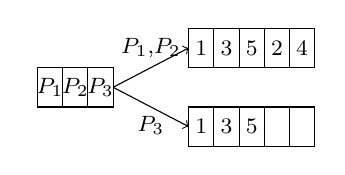
\begin{tikzpicture}[font=\footnotesize]
    % Define the width and height of the rectangles
    \def\rectwidth{0.32}
    \def\rectheight{0.5}
    \def\listdist{1.6}
        
    % Draw the queue
    \draw (-\rectwidth,0) rectangle (\rectwidth,\rectheight);
    \node at (-\rectwidth/2,\rectheight/2) {$P_1$};

    \draw (0,0) rectangle (\rectwidth,\rectheight);
    \node at (\rectwidth/2,\rectheight/2) {$P_2$};

    \draw (\rectwidth,0) rectangle (2*\rectwidth,\rectheight);
    \node at (\rectwidth+\rectwidth/2,\rectheight/2) {$P_3$};
%     
    % Add arrows from the head of the queue
    \draw[->] (2*\rectwidth,\rectheight/2) -- (\listdist,3*\rectheight/2) node[midway, above] {$P_1$,$P_2$};
    \draw[->] (2*\rectwidth,\rectheight/2) -- (\listdist,-\rectheight/2) node[midway, below] {$P_3$};
  
    \foreach \x in {0,1,2,3,4} {
      \draw (\listdist+\x*\rectwidth,\rectheight) rectangle (\listdist+\x*\rectwidth+\rectwidth,2*\rectheight);
      \draw (\listdist+\x*\rectwidth,-\rectheight) rectangle (\listdist+\x*\rectwidth+\rectwidth,0);
    }

    \node at (\listdist+\rectwidth/2,-\rectheight/2) {1};
    \node at (\listdist+\rectwidth+\rectwidth/2,-\rectheight/2) {3};
    \node at (\listdist+2*\rectwidth+\rectwidth/2,-\rectheight/2) {5};

    \node at (\listdist+\rectwidth/2,3*\rectheight/2) {1};
    \node at (\listdist+\rectwidth+\rectwidth/2,3*\rectheight/2) {3};
    \node at (\listdist+2*\rectwidth+\rectwidth/2,3*\rectheight/2) {5};
    \node at (\listdist+3*\rectwidth+\rectwidth/2,3*\rectheight/2) {2};
    \node at (\listdist+4*\rectwidth+\rectwidth/2,3*\rectheight/2) {4};
\end{tikzpicture}

%%% Local Variables:
%%% mode: latex
%%% TeX-master: "../distributed_mrf"
%%% End:

    \label{fig:active-rule-imperfect-lb}
  }
  % \hspace{-1em}
  \subfloat[][Perfect separation]{
    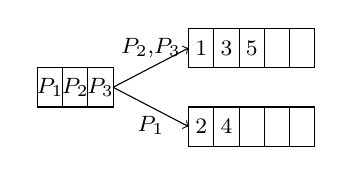
\begin{tikzpicture}[font=\footnotesize]
    % Define the width and height of the rectangles
    \def\rectwidth{0.32}
    \def\rectheight{0.5}
    \def\listdist{1.6}
        
    % Draw the queue
    \draw (-\rectwidth,0) rectangle (\rectwidth,\rectheight);
    \node at (-\rectwidth/2,\rectheight/2) {$P_1$};

    \draw (0,0) rectangle (\rectwidth,\rectheight);
    \node at (\rectwidth/2,\rectheight/2) {$P_2$};

    \draw (\rectwidth,0) rectangle (2*\rectwidth,\rectheight);
    \node at (\rectwidth+\rectwidth/2,\rectheight/2) {$P_3$};
%     
    % Add arrows from the head of the queue
    \draw[->] (2*\rectwidth,\rectheight/2) -- (\listdist,3*\rectheight/2) node[midway, above] {$P_2$,$P_3$};
    \draw[->] (2*\rectwidth,\rectheight/2) -- (\listdist,-\rectheight/2) node[midway, below] {$P_1$};

    \foreach \x in {0,1,2,3,4} {
      \draw (\listdist+\x*\rectwidth,\rectheight) rectangle (\listdist+\x*\rectwidth+\rectwidth,2*\rectheight);
      \draw (\listdist+\x*\rectwidth,-\rectheight) rectangle (\listdist+\x*\rectwidth+\rectwidth,0);
    }

    \node at (\listdist+\rectwidth/2,-\rectheight/2) {2};
    \node at (\listdist+\rectwidth+\rectwidth/2,-\rectheight/2) {4};
    \node at (\listdist+2*\rectwidth+\rectwidth/2,-\rectheight/2) {};

    \node at (\listdist+\rectwidth/2,3*\rectheight/2) {1};
    \node at (\listdist+\rectwidth+\rectwidth/2,3*\rectheight/2) {3};
    \node at (\listdist+2*\rectwidth+\rectwidth/2,3*\rectheight/2) {5};
    \node at (\listdist+3*\rectwidth+\rectwidth/2,3*\rectheight/2) {};
    \node at (\listdist+4*\rectwidth+\rectwidth/2,3*\rectheight/2) {};
\end{tikzpicture}

%%% Local Variables:
%%% mode: latex
%%% TeX-master: "../distributed_mrf"
%%% End:

    \label{fig:active-rule-perfect-lb}
  }
  \caption{Locality-boosting load balancing over packet sequence $P_1$ (matching rule 4 of the sample classifier in Fig.~\ref{fig:class-sample}) followed by $P_2$ and $P_3$ (both matching rule 5): (a) hash-based load balancing may assign $P_2$ and $P_3$ to different workers so that both will have to keep the dependency list $5\to 3\to 1$ in the active rule set, (b) perfect separation sends $P_1$ and $P_2$ to the same worker, yielding minimal active rule sets.}
  \label{fig:active-set-lb}
\end{figure}

% \subsection{Implementation}
% \label{sec:sa-nf-tables-impl}

\subsection{Reproducing superlinear speedup}
\label{sec:sa-nf-tables-eval}

We conducted several experiments with the distributed self-adjusting packet classifier combined with the hash-based RSS load balancer. Our goal was to understand whether superlinear scaling can be robustly reproduced on a real network application using real packet I/O. % Further,  we aim to determine the conditions (rule sets, flow size, etc) under which it emerges.

\begin{figure*}[t]
  \centering
  \subfloat[][acl1]{
    \pgfplotsset{
  RatePlot/.style = {
    tick pos = left,
    xtick align=outside,
    ytick align=outside,
    xlabel near ticks,
    ylabel near ticks,
    width=.4\textwidth,
    height=.3\textwidth,
    legend pos = north west,
    legend cell align=left,
    ylabel = {Throughput [Mpps]},
    xlabel = {number of CPU cores},
    xmin=1, xmax=32,
    ymin=0,
  },
  SpeedupPlot/.style = {
    RatePlot,
    ylabel={Speedup},
  },
  ClassBenchGroupPlot/.style = {
    group/group size = 1 by 2,
    group/horizontal sep = 0pt,
    group/vertical sep = 28pt,
  },
  ClassBenchRatePlot/.style = {
    RatePlot
  },
  ClassBenchSpeedupPlot/.style = {
    SpeedupPlot,
  }
}

%%% Local Variables:
%%% mode: latex
%%% TeX-master: "../distributed_mrf.tex"
%%% End:


\begin{tikzpicture}

 \begin{groupplot}[ClassBenchGroupPlot]

  \nextgroupplot[ClassBenchSpeedupPlot]

  \addplot coordinates {
     (1, 1.00000)
     (2, 2.01275)
     (3, 2.99326)
     (4, 4.03999)
     (5, 5.02312)
     (6, 6.02253)
     (7, 7.01021)
     (8, 8.04299)
     (9, 9.02064)
     (10, 10.03534)
     (11, 11.10694)
     (12, 12.08788)
     (13, 13.07358)
     (14, 14.01179)
     (15, 15.05161)
     (16, 16.13280)
     (17, 17.14857)
     (18, 18.07133)
     (19, 19.04549)
     (20, 20.20622)
     (21, 21.20803)
     (22, 22.09785)
     (23, 23.04393)
     (24, 24.23765)
     (25, 25.17218)
     (26, 26.28756)
     (27, 27.06453)
     (28, 27.74060)
     (29, 28.61572)
     (30, 29.48150)
     (31, 30.28735)
     (32, 31.37051)
     (33, 31.31105)
     (34, 31.46892)
     (35, 31.41659)
     (36, 31.50497)
     (37, 31.88759)
     (38, 31.98595)
     (39, 32.18120)
     (40, 32.26755)
     (41, 32.51116)
     (42, 32.68041)
     (43, 33.08639)
     (44, 33.06703)
     (45, 33.14436)
     (46, 33.23806)
     (47, 33.46593)
     (48, 33.40066)
     (49, 33.61066)
     (50, 33.73653)
     (51, 34.05734)
     (52, 34.13124)
     (53, 34.31725)
     (54, 34.47786)
     (55, 34.61957)
     (56, 34.64922)
     (57, 34.57655)
     (58, 34.92709)
     (59, 34.83238)
     (60, 35.29259)
     (61, 35.46089)
     (62, 35.39285)
     (63, 35.38630)
    };
    \addlegendentry{Static}

  \addplot coordinates {
     (1, 1.00000)
     (2, 2.78880)
     (3, 5.34148)
     (4, 8.50314)
     (5, 12.18752)
     (6, 16.29228)
     (7, 20.91828)
     (8, 25.42996)
     (9, 30.76640)
     (10, 35.64435)
     (11, 42.18526)
     (12, 47.99208)
     (13, 54.94981)
     (14, 61.30928)
     (15, 67.57976)
     (16, 76.48709)
     (17, 84.80360)
     (18, 88.83299)
     (19, 98.87346)
     (20, 105.97422)
     (21, 117.95420)
     (22, 124.30595)
     (23, 130.33294)
     (24, 141.99362)
     (25, 151.39788)
     (26, 164.00849)
     (27, 169.80391)
     (28, 181.86091)
     (29, 191.72184)
     (30, 196.66672)
     (31, 210.59534)
     (32, 225.16466)
     (33, 224.40485)
     (34, 229.31071)
     (35, 229.13107)
     (36, 236.10585)
     (37, 249.26799)
     (38, 243.55203)
     (39, 246.00255)
     (40, 256.27063)
     (41, 260.25177)
     (42, 266.14283)
     (43, 269.95816)
     (44, 277.40640)
     (45, 281.26218)
     (46, 280.08708)
     (47, 285.01959)
     (48, 289.29034)
     (49, 290.48724)
     (50, 294.05818)
     (51, 298.84372)
     (52, 304.31674)
     (53, 306.37411)
     (54, 305.79708)
     (55, 306.30851)
     (56, 309.33107)
     (57, 313.83119)
     (58, 320.11412)
     (59, 329.67394)
     (60, 323.96154)
     (61, 336.04423)
     (62, 334.62710)
     (63, 342.45456)
    };
    \addlegendentry{Self-adjusting}


  \nextgroupplot[ClassBenchRatePlot]

    \addplot coordinates {
      (1, 0.046539629713245)
      (2, 0.093672584131231)
      (3, 0.1393051523559)
      (4, 0.18801951171016)
      (5, 0.2337741675624)
      (6, 0.28028621268916)
      (7, 0.32625249458415)
      (8, 0.37431778626937)
      (9, 0.41981712674747)
      (10, 0.46704104588755)
      (11, 0.51691309033259)
      (12, 0.56256543220967)
      (13, 0.60843936704226)
      (14, 0.65210352613963)
      (15, 0.70049618756688)
      (16, 0.75081434963534)
      (17, 0.79808802554201)
      (18, 0.84103282307131)
      (19, 0.8863702768161)
      (20, 0.9403901302883)
      (21, 0.98701389451984)
      (22, 1.0284257030863)
      (23, 1.0724561987193)
      (24, 1.1280112041682)
      (25, 1.1715041448177)
      (26, 1.2234130913758)
      (27, 1.2595730640873)
      (28, 1.2910370796756)
      (29, 1.3317647863544)
      (30, 1.3720579499166)
      (31, 1.4095619991636)
      (32, 1.4599720329117)
      (33, 1.4572048750005)
      (34, 1.4645519240141)
      (35, 1.4621164290821)
      (36, 1.4662297251988)
      (37, 1.4840364875665)
      (38, 1.4886142627512)
      (39, 1.4977010671677)
      (40, 1.5017199796616)
      (41, 1.513057464791)
      (42, 1.5209341329062)
      (43, 1.5398284158632)
      (44, 1.5389273111143)
      (45, 1.5425261198347)
      (46, 1.5468869141326)
      (47, 1.5574918678777)
      (48, 1.5544544573799)
      (49, 1.5642275725289)
      (50, 1.570085466313)
      (51, 1.5850162120482)
      (52, 1.5884550498825)
      (53, 1.5971119199612)
      (54, 1.6045867927364)
      (55, 1.6111820668819)
      (56, 1.6125620968556)
      (57, 1.6091796950591)
      (58, 1.625494043245)
      (59, 1.6210858597396)
      (60, 1.6425038639144)
      (61, 1.6503368924279)
      (62, 1.6471702537073)
      (63, 1.646865499047)
    };
    %\addlegendentry{Static}

    \addplot coordinates {
      (1, 0.032711671064758)
      (2, 0.091226367386569)
      (3, 0.17472861741391)
      (4, 0.27815189405222)
      (5, 0.39867428595652)
      (6, 0.53294756137404)
      (7, 0.68427196615884)
      (8, 0.83185664878198)
      (9, 1.0064203293998)
      (10, 1.1659863048086)
      (11, 1.3799504801709)
      (12, 1.5699010587605)
      (13, 1.7975000467864)
      (14, 2.0055291591319)
      (15, 2.2106470134093)
      (16, 2.5020206145042)
      (17, 2.7740673059055)
      (18, 2.9058754936516)
      (19, 3.2343161023274)
      (20, 3.4665937520818)
      (21, 3.8584788645415)
      (22, 4.0662555102297)
      (23, 4.2634082896897)
      (24, 4.6448485014523)
      (25, 4.9524775583613)
      (26, 5.364991630779)
      (27, 5.5545694871632)
      (28, 5.9489741357534)
      (29, 6.271541634084)
      (30, 6.433297006678)
      (31, 6.8889255847637)
      (32, 7.3655123135189)
      (33, 7.340657797016)
      (34, 7.5011366031331)
      (35, 7.4952600759246)
      (36, 7.7234167470822)
      (37, 8.1539723522886)
      (38, 7.9669939347613)
      (39, 8.0471546196194)
      (40, 8.3830405627332)
      (41, 8.5132704352016)
      (42, 8.7059768571641)
      (43, 8.8307824941431)
      (44, 9.0744269109974)
      (45, 9.2005560451181)
      (46, 9.162116552901)
      (47, 9.3234670053344)
      (48, 9.4631704141204)
      (49, 9.5023229923151)
      (50, 9.6191344074074)
      (51, 9.7756773452302)
      (52, 9.954709011936)
      (53, 10.022009206075)
      (54, 10.00313342368)
      (55, 10.019863323224)
      (56, 10.118736180131)
      (57, 10.265942613862)
      (58, 10.471467947096)
      (59, 10.784185365095)
      (60, 10.597323449753)
      (61, 10.992568407591)
      (62, 10.946211746648)
      (63, 11.20226094469)
    };
    %\addlegendentry{Self-adjusting}

  \end{groupplot}

  % Inset delay figure
  %\begin{axis}[
  RatePlot,
  xshift = 2.5pt,
  yshift = -32.5pt,
  width=87.5pt,
  height=65pt,
  ylabel shift = -5 pt,
  xlabel shift = -5 pt,
  xlabel = {\# CPU cores},
  ylabel = {Delay [ms]},
  major tick length = 1.5,
  minor tick length = .75,
  xtick align = inside,
  ytick align = inside,
  ytick pos = right,
  xlabel shift = -5pt,
  xticklabel shift = -2pt,
  ylabel shift = -5pt,
  yticklabel shift = -2pt,
  yticklabel pos = right,
  ticklabel style = {font = \tiny},
  label style = {font = \tiny},
  font = \tiny,
  ]

  \addplot[StaticMarkSmall] coordinates {
    (1, 11.5246859)
    (2, 13.0414406)
    (3, 12.0516008)
    (4, 12.4346342)
    (5, 12.7136874)
    (6, 12.4196939)
    (7, 12.9454364)
    (8, 12.5504689)
    (9, 13.1494149)
    (10, 13.4371564)
    (11, 13.2305652)
    (12, 13.4584262)
    (13, 13.6475760)
    (14, 13.9229871)
    (15, 13.6530165)
    (16, 13.5959664)
    (17, 13.7759351)
    (18, 13.9005972)
    (19, 13.8574247)
    (20, 13.9209600)
    (21, 14.0194501)
    (22, 14.0310233)
    (23, 14.1952436)
    (24, 13.8615738)
    (25, 13.7690495)
    (26, 13.6904902)
    (27, 13.9852999)
    (28, 14.0805306)
    (29, 14.0971204)
    (30, 14.0061332)
    (31, 13.6011743)
    (32, 13.4245527)
    (33, 14.0842828)
    (34, 14.1634843)
    (35, 14.4694397)
    (36, 14.2107712)
    (37, 14.6166717)
    (38, 14.4130623)
    (39, 14.3040049)
    (40, 13.4596624)
    (41, 14.0578499)
    (42, 14.2140139)
    (43, 14.4488030)
    (44, 14.3561524)
    (45, 14.2936769)
    (46, 14.4158717)
    (47, 14.6920556)
    (48, 14.4894246)
    (49, 14.5674845)
    (50, 14.6061373)
    (51, 14.2901432)
    (52, 14.3238256)
    (53, 14.3649980)
    (54, 14.3366655)
    (55, 14.5369478)
    (56, 14.8161641)
    (57, 14.6632713)
    (58, nan)
    (59, 14.6380668)
    (60, 13.9192529)
    (61, 13.9991509)
    (62, 13.7683118)
    (63, nan)
  };

  \addplot[SelfAdjustingMarkSmall] coordinates {
    (1, 13.7504560)
    (2, 12.8632773)
    (3, 10.5175126)
    (4, 10.3660933)
    (5, 09.0034255)
    (6, 07.9318335)
    (7, 07.8026594)
    (8, 06.3111752)
    (9, 06.5644485)
    (10, 06.2939857)
    (11, 05.5898275)
    (12, 05.3072441)
    (13, 05.6942094)
    (14, 04.9724582)
    (15, 04.1699062)
    (16, 03.9506734)
    (17, 04.2641513)
    (18, 04.4839685)
    (19, 03.7867425)
    (20, 03.8697160)
    (21, 03.6709087)
    (22, 03.5707060)
    (23, 03.7592740)
    (24, 03.7324230)
    (25, 03.0875692)
    (26, 03.4737530)
    (27, 02.6244803)
    (28, 02.5924367)
    (29, 02.2520316)
    (30, 02.9590999)
    (31, 02.1526739)
    (32, 02.1813730)
    (33, 02.5701373)
    (34, 02.7773967)
    (35, 03.8287018)
    (36, 03.0827487)
    (37, 02.4387644)
    (38, 02.6892771)
    (39, 02.8402511)
    (40, 02.8046372)
    (41, 02.3915482)
    (42, 02.0204283)
    (43, 02.6570434)
    (44, 02.9146742)
    (45, 02.6903529)
    (46, 04.1966236)
    (47, 03.9124022)
    (48, 03.1979138)
    (49, 01.8601223)
    (50, 0.31112418)
    (51, 0.19742585)
    (52, 0.16013978)
    (53, 0.07419928)
    (54, 0.20887176)
    (55, 0.12476317)
    (56, 0.12985358)
    (57, 0.20131270)
    (58, 0.09126601)
    (59, 0.24982249)
    (60, 0.16912486)
    (61, 0.12356464)
    (62, 0.06734899)
    (63, 0.28888528)
  };
\end{axis}


\end{tikzpicture}

    \label{fig:classbench-acl1}
  }
  \hspace{-1em}
  \subfloat[][ipc1]{
    \pgfplotsset{
  RatePlot/.style = {
    tick pos = left,
    xtick align=outside,
    ytick align=outside,
    xlabel near ticks,
    ylabel near ticks,
    width=.4\textwidth,
    height=.3\textwidth,
    legend pos = north west,
    legend cell align=left,
    ylabel = {Throughput [Mpps]},
    xlabel = {number of CPU cores},
    xmin=1, xmax=32,
    ymin=0,
  },
  SpeedupPlot/.style = {
    RatePlot,
    ylabel={Speedup},
  },
  ClassBenchGroupPlot/.style = {
    group/group size = 1 by 2,
    group/horizontal sep = 0pt,
    group/vertical sep = 28pt,
  },
  ClassBenchRatePlot/.style = {
    RatePlot
  },
  ClassBenchSpeedupPlot/.style = {
    SpeedupPlot,
  }
}

%%% Local Variables:
%%% mode: latex
%%% TeX-master: "../distributed_mrf.tex"
%%% End:


\begin{tikzpicture}

 \begin{groupplot}[ClassBenchGroupPlot]

  \nextgroupplot[ClassBenchSpeedupPlot]

  \addplot coordinates {
     (1, 1.00000)
     (2, 1.99904)
     (3, 2.89529)
     (4, 3.94680)
     (5, 4.94148)
     (6, 5.74940)
     (7, 6.84421)
     (8, 7.87120)
     (9, 8.68609)
     (10, 9.62543)
     (11, 10.76151)
     (12, 11.59969)
     (13, 12.48071)
     (14, 13.37427)
     (15, 14.31106)
     (16, 15.34732)
     (17, 16.21912)
     (18, 17.26689)
     (19, 18.25517)
     (20, 18.99125)
     (21, 20.10330)
     (22, 21.12825)
     (23, 21.98638)
     (24, 23.02527)
     (25, 23.99193)
     (26, 25.00409)
     (27, 25.96916)
     (28, 26.76306)
     (29, 27.67258)
     (30, 28.77140)
     (31, 29.50573)
     (32, 30.37490)
     (33, 30.40629)
     (34, 30.64074)
     (35, 30.72365)
     (36, 31.37580)
     (37, 31.42249)
     (38, 31.81717)
     (39, 32.17639)
     (40, 32.28154)
     (41, 32.51125)
     (42, 32.95661)
     (43, 33.02789)
     (44, 33.48791)
     (45, 34.04567)
     (46, 34.06134)
     (47, 34.66463)
     (48, 34.72688)
     (49, 35.10103)
     (50, 35.47690)
     (51, 35.60816)
     (52, 35.97768)
     (53, 36.07897)
     (54, 36.55234)
     (55, 36.74071)
     (56, 37.00593)
     (57, 37.28585)
     (58, 37.56701)
     (59, 37.85790)
     (60, 38.13999)
     (61, 38.65728)
     (62, 38.72069)
     (63, 38.99848)
    };
    \addlegendentry{Static}

  \addplot coordinates {
     (1, 1.00000)
     (2, 2.20256)
     (3, 3.66848)
     (4, 5.28803)
     (5, 7.07860)
     (6, 9.02878)
     (7, 10.92263)
     (8, 12.96272)
     (9, 15.22643)
     (10, 17.22539)
     (11, 19.33919)
     (12, 21.74296)
     (13, 24.06457)
     (14, 26.16635)
     (15, 28.95934)
     (16, 30.80881)
     (17, 33.36339)
     (18, 35.92651)
     (19, 37.90040)
     (20, 40.60494)
     (21, 43.38436)
     (22, 46.13333)
     (23, 48.23023)
     (24, 51.33538)
     (25, 53.98739)
     (26, 56.26039)
     (27, 59.36582)
     (28, 61.28844)
     (29, 65.46223)
     (30, 67.96489)
     (31, 69.39216)
     (32, 72.02270)
     (33, 73.73031)
     (34, 74.33798)
     (35, 75.79911)
     (36, 78.07703)
     (37, 78.74681)
     (38, 78.92463)
     (39, 83.23712)
     (40, 81.81416)
     (41, 83.07275)
     (42, 85.40033)
     (43, 87.80475)
     (44, 89.72449)
     (45, 89.83877)
     (46, 89.94273)
     (47, 92.81415)
     (48, 93.06880)
     (49, 95.82243)
     (50, 96.56137)
     (51, 98.81827)
     (52, 98.02214)
     (53, 102.84065)
     (54, 103.14348)
     (55, 102.71015)
     (56, 103.91244)
     (57, 103.91456)
     (58, 110.49607)
     (59, 112.25616)
     (60, 111.94357)
     (61, 115.83462)
     (62, 114.89240)
     (63, 115.08863)
    };
    \addlegendentry{Self-adjusting}


  \nextgroupplot[ClassBenchRatePlot]

    \addplot coordinates {
      (1, 0.031744111665511)
      (2, 0.06345764248803)
      (3, 0.091908519541636)
      (4, 0.12528766365938)
      (5, 0.15686304594011)
      (6, 0.18250956925555)
      (7, 0.21726343486567)
      (8, 0.24986432095669)
      (9, 0.27573229304931)
      (10, 0.30555056652382)
      (11, 0.34161460030774)
      (12, 0.36822186805517)
      (13, 0.39618898479011)
      (14, 0.42455421455473)
      (15, 0.45429173415525)
      (16, 0.48718705524847)
      (17, 0.51486159839532)
      (18, 0.54812209288819)
      (19, 0.57949418947039)
      (20, 0.60286035824686)
      (21, 0.63816150612146)
      (22, 0.67069744081536)
      (23, 0.69793805530304)
      (24, 0.73091662482903)
      (25, 0.76160264715354)
      (26, 0.79373269598525)
      (27, 0.82436782385871)
      (28, 0.84956963537846)
      (29, 0.87844154226898)
      (30, 0.91332255008854)
      (31, 0.93663321831887)
      (32, 0.96422433146812)
      (33, 0.96522063738741)
      (34, 0.97266295711053)
      (35, 0.97529501211155)
      (36, 0.99599704950763)
      (37, 0.9974789718364)
      (38, 1.0100078956506)
      (39, 1.0214108255887)
      (40, 1.0247489335771)
      (41, 1.0320407243525)
      (42, 1.0461783410233)
      (43, 1.0484410263942)
      (44, 1.0630439417362)
      (45, 1.0807493982743)
      (46, 1.0812469142839)
      (47, 1.1003979788613)
      (48, 1.1023740588795)
      (49, 1.114251025749)
      (50, 1.1261827795326)
      (51, 1.1303495040476)
      (52, 1.1420795825023)
      (53, 1.1452948199886)
      (54, 1.1603215255264)
      (55, 1.1663011271238)
      (56, 1.1747203713183)
      (57, 1.1836061503951)
      (58, 1.1925312282163)
      (59, 1.2017655298065)
      (60, 1.2107201289644)
      (61, 1.2271411601153)
      (62, 1.2291540532193)
      (63, 1.2379719857676)
    };
    %\addlegendentry{Static}

    \addplot coordinates {
      (1, 0.018889987135068)
      (2, 0.041606239750658)
      (3, 0.069297553101307)
      (4, 0.09989082130905)
      (5, 0.13371469324804)
      (6, 0.17055354254507)
      (7, 0.20632828893924)
      (8, 0.24486570461986)
      (9, 0.28762697309928)
      (10, 0.32538748583933)
      (11, 0.36531712499108)
      (12, 0.41072423416958)
      (13, 0.45457945262613)
      (14, 0.49428201504977)
      (15, 0.54704156833915)
      (16, 0.58197799770858)
      (17, 0.63023392021364)
      (18, 0.67865132429634)
      (19, 0.71593800237838)
      (20, 0.76702670262749)
      (21, 0.81953000032308)
      (22, 0.87145801355135)
      (23, 0.91106846222972)
      (24, 0.96972458688005)
      (25, 1.0198211188854)
      (26, 1.0627580921815)
      (27, 1.1214195184789)
      (28, 1.1577377491515)
      (29, 1.2365806896474)
      (30, 1.2838558959822)
      (31, 1.3108169705898)
      (32, 1.3605078081155)
      (33, 1.3927646148772)
      (34, 1.4042435625386)
      (35, 1.4318442480682)
      (36, 1.4748740145751)
      (37, 1.4875261749455)
      (38, 1.4908852601269)
      (39, 1.5723481148306)
      (40, 1.545468447653)
      (41, 1.5692432165363)
      (42, 1.6132111202603)
      (43, 1.6586305311713)
      (44, 1.6948944717015)
      (45, 1.6970531644274)
      (46, 1.6990170088985)
      (47, 1.753258037858)
      (48, 1.7580683551754)
      (49, 1.810084485413)
      (50, 1.8240430490041)
      (51, 1.8666759363908)
      (52, 1.8516369793844)
      (53, 1.9426585570425)
      (54, 1.9483789317255)
      (55, 1.9401934934174)
      (56, 1.9629046074725)
      (57, 1.9629446910417)
      (58, 2.0872693483339)
      (59, 2.1205175033934)
      (60, 2.1146125661818)
      (61, 2.1881144974859)
      (62, 2.1703159284934)
      (63, 2.1740227160904)
    };
    %\addlegendentry{Self-adjusting}

  \end{groupplot}
\end{tikzpicture}

    \label{fig:classbench-ipc1}
  }
  \hspace{-1em}
  \subfloat[][fw1]{
    \pgfplotsset{
  RatePlot/.style = {
    tick pos = left,
    xtick align=outside,
    ytick align=outside,
    xlabel near ticks,
    ylabel near ticks,
    width=.4\textwidth,
    height=.3\textwidth,
    legend pos = north west,
    legend cell align=left,
    ylabel = {Throughput [Mpps]},
    xlabel = {number of CPU cores},
    xmin=1, xmax=32,
    ymin=0,
  },
  SpeedupPlot/.style = {
    RatePlot,
    ylabel={Speedup},
  },
  ClassBenchGroupPlot/.style = {
    group/group size = 1 by 2,
    group/horizontal sep = 0pt,
    group/vertical sep = 28pt,
  },
  ClassBenchRatePlot/.style = {
    RatePlot
  },
  ClassBenchSpeedupPlot/.style = {
    SpeedupPlot,
  }
}

%%% Local Variables:
%%% mode: latex
%%% TeX-master: "../distributed_mrf.tex"
%%% End:


\begin{tikzpicture}

 \begin{groupplot}[ClassBenchGroupPlot]

  \nextgroupplot[ClassBenchSpeedupPlot, ytick distance={25},]

  \addplot[StaticMark,each nth point={2}] coordinates {
     (1, 1.00000)
     (2, 2.00642)
     (3, 3.00227)
     (4, 3.98526)
     (5, 4.97784)
     (6, 5.97126)
     (7, 6.95429)
     (8, 7.92904)
     (9, 8.95196)
     (10, 9.95693)
     (11, 10.95708)
     (12, 11.90737)
     (13, 12.98807)
     (14, 13.89798)
     (15, 14.90286)
     (16, 15.90926)
     (17, 16.87838)
     (18, 17.88937)
     (19, 18.83991)
     (20, 19.79596)
     (21, 20.79066)
     (22, 21.78117)
     (23, 22.95279)
     (24, 23.92195)
     (25, 24.87083)
     (26, 25.97827)
     (27, 26.83614)
     (28, 27.48385)
     (29, 28.32628)
     (30, 29.25493)
     (31, 30.03297)
     (32, 30.49489)
     (33, 30.87020)
     (34, 31.08683)
     (35, 31.13049)
     (36, 31.37795)
     (37, 31.55764)
     (38, 31.83831)
     (39, 31.74457)
     (40, 31.98458)
     (41, 32.29963)
     (42, 32.32307)
     (43, 32.32149)
     (44, 32.63861)
     (45, 32.67067)
     (46, 32.75227)
     (47, 32.93674)
     (48, 32.95525)
     (49, 33.01142)
     (50, 33.21486)
     (51, 33.49748)
     (52, 33.71485)
     (53, 33.94554)
     (54, 33.82370)
     (55, 34.05714)
     (56, 34.42454)
     (57, 34.30365)
     (58, 34.57126)
     (59, 34.62224)
     (60, 34.84287)
     (61, 34.92018)
     (62, 35.08595)
     (63, 35.27453)
    };
    \addlegendentry{Static}

  \addplot[SelfAdjustingMark,each nth point={2}] coordinates {
     (1, 1.00000)
     (2, 2.10620)
     (3, 3.32994)
     (4, 4.60646)
     (5, 6.04220)
     (6, 7.52206)
     (7, 8.85721)
     (8, 10.44222)
     (9, 11.97781)
     (10, 13.58400)
     (11, 15.12528)
     (12, 16.83646)
     (13, 18.62258)
     (14, 19.90959)
     (15, 22.03945)
     (16, 23.29472)
     (17, 25.05463)
     (18, 27.26867)
     (19, 28.36004)
     (20, 30.56113)
     (21, 32.33906)
     (22, 33.74235)
     (23, 35.46088)
     (24, 37.95365)
     (25, 39.50008)
     (26, 42.13974)
     (27, 43.99437)
     (28, 45.11863)
     (29, 47.74894)
     (30, 50.61731)
     (31, 51.52214)
     (32, 52.83959)
     (33, 53.56519)
     (34, 54.73500)
     (35, 56.08416)
     (36, 56.88490)
     (37, 58.82567)
     (38, 57.26452)
     (39, 61.12304)
     (40, 60.10926)
     (41, 61.54647)
     (42, 60.44772)
     (43, 65.14732)
     (44, 62.42518)
     (45, 64.11267)
     (46, 64.33649)
     (47, 65.25661)
     (48, 66.65516)
     (49, 67.07342)
     (50, 69.85434)
     (51, 68.17294)
     (52, 70.97795)
     (53, 71.39927)
     (54, 74.81633)
     (55, 74.06910)
     (56, 75.78303)
     (57, 73.92442)
     (58, 78.45669)
     (59, 78.68256)
     (60, 81.34688)
     (61, 79.42674)
     (62, 82.14868)
     (63, 81.65074)
    };
    \addlegendentry{Self-adjusting}


    \nextgroupplot[ClassBenchRatePlot, ytick distance={.25},]

    \addplot[StaticMark,each nth point={2}] coordinates {
      (1, 0.046175337275456)
      (2, 0.09264702209592)
      (3, 0.13863104867912)
      (4, 0.18402089749063)
      (5, 0.22985352206762)
      (6, 0.27572504514474)
      (7, 0.32111657076421)
      (8, 0.36612603036957)
      (9, 0.41335992529034)
      (10, 0.45976448979103)
      (11, 0.50594685313329)
      (12, 0.54982685620667)
      (13, 0.59972869147124)
      (14, 0.64174406455464)
      (15, 0.68814442112783)
      (16, 0.73461527598681)
      (17, 0.77936467117974)
      (18, 0.82604754443381)
      (19, 0.86993899027163)
      (20, 0.91408535287356)
      (21, 0.96001563210835)
      (22, 1.0057528255294)
      (23, 1.0598530159052)
      (24, 1.1046042462612)
      (25, 1.1484188298822)
      (26, 1.1995551986021)
      (27, 1.2391676499915)
      (28, 1.2690762528259)
      (29, 1.3079755350045)
      (30, 1.3508561030092)
      (31, 1.3867826333745)
      (32, 1.4081119335249)
      (33, 1.4254417984352)
      (34, 1.4354447905783)
      (35, 1.4374608756753)
      (36, 1.4488872783868)
      (37, 1.457184487247)
      (38, 1.4701448721321)
      (39, 1.4658163675455)
      (40, 1.4768986840629)
      (41, 1.4914464990695)
      (42, 1.4925285957533)
      (43, 1.4924556002395)
      (44, 1.5070988035406)
      (45, 1.5085793445279)
      (46, 1.5123468886761)
      (47, 1.5208652043167)
      (48, 1.5217199585225)
      (49, 1.5243135939772)
      (50, 1.5337073923782)
      (51, 1.5467576297889)
      (52, 1.5567944652189)
      (53, 1.5674465598604)
      (54, 1.561820787017)
      (55, 1.5725999883676)
      (56, 1.5895646786313)
      (57, 1.5839824554285)
      (58, 1.5963394180261)
      (59, 1.5986934308387)
      (60, 1.6088812904173)
      (61, 1.6124509802072)
      (62, 1.6201056318048)
      (63, 1.6288131272854)
    };
    %\addlegendentry{Static}

    \addplot[SelfAdjustingMark,each nth point={2}] coordinates {
      (1, 0.026644006858161)
      (2, 0.056117557869066)
      (3, 0.088723041020338)
      (4, 0.12273458673186)
      (5, 0.16098834116769)
      (6, 0.20041792048914)
      (7, 0.23599149569214)
      (8, 0.27822253191441)
      (9, 0.31913689382905)
      (10, 0.36193211309214)
      (11, 0.40299813009226)
      (12, 0.44859084774872)
      (13, 0.49618009062294)
      (14, 0.53047118514086)
      (15, 0.58721926451141)
      (16, 0.62066461989621)
      (17, 0.66755582214289)
      (18, 0.72654675580445)
      (19, 0.75562501559322)
      (20, 0.81427091549728)
      (21, 0.86164203247128)
      (22, 0.89903130126662)
      (23, 0.94481992091986)
      (24, 1.0112373794178)
      (25, 1.0524403251209)
      (26, 1.1227715208184)
      (27, 1.1721861953998)
      (28, 1.202140956169)
      (29, 1.2722232054971)
      (30, 1.3486478783407)
      (31, 1.3727562816561)
      (32, 1.4078583915456)
      (33, 1.4271911802559)
      (34, 1.4583596377024)
      (35, 1.4943067887155)
      (36, 1.5156416288099)
      (37, 1.5673514418731)
      (38, 1.5257563653458)
      (39, 1.6285626741519)
      (40, 1.6015515358324)
      (41, 1.6398446846539)
      (42, 1.6105695090346)
      (43, 1.7357855482578)
      (44, 1.663257048135)
      (45, 1.7082183696376)
      (46, 1.7141818711466)
      (47, 1.7386976353862)
      (48, 1.7759606689769)
      (49, 1.7871046751784)
      (50, 1.8611995228113)
      (51, 1.8164003584035)
      (52, 1.8911369475636)
      (53, 1.9023625888079)
      (54, 1.9934069178642)
      (55, 1.9734976870415)
      (56, 2.0191634605762)
      (57, 1.9696427700865)
      (58, 2.0904006165687)
      (59, 2.0964187625424)
      (60, 2.1674069288648)
      (61, 2.1162466149076)
      (62, 2.188770066379)
      (63, 2.1755028772937)
    };
    %\addlegendentry{Self-adjusting}

  \end{groupplot}
\end{tikzpicture}

    \label{fig:classbench-fw1}
  }
  \hspace{-1em}
  \subfloat[][Synthetic traffic]{
    \pgfplotsset{
  RatePlot/.style = {
    tick pos = left,
    xtick align=outside,
    ytick align=outside,
    xlabel near ticks,
    ylabel near ticks,
    width=.4\textwidth,
    height=.3\textwidth,
    legend pos = north west,
    legend cell align=left,
    ylabel = {Throughput [Mpps]},
    xlabel = {number of CPU cores},
    xmin=1, xmax=32,
    ymin=0,
  },
  SpeedupPlot/.style = {
    RatePlot,
    ylabel={Speedup},
  },
  ClassBenchGroupPlot/.style = {
    group/group size = 1 by 2,
    group/horizontal sep = 0pt,
    group/vertical sep = 28pt,
  },
  ClassBenchRatePlot/.style = {
    RatePlot
  },
  ClassBenchSpeedupPlot/.style = {
    SpeedupPlot,
  }
}

%%% Local Variables:
%%% mode: latex
%%% TeX-master: "../distributed_mrf.tex"
%%% End:


\begin{tikzpicture}
  \begin{axis}[SpeedupPlot]

    \addplot coordinates {
     (1, 1.00000)
     (2, 3.95295)
     (3, 8.92334)
     (4, 14.46385)
     (5, 21.54861)
     (6, 31.60320)
     (7, 41.12957)
     (8, 50.19947)
     (9, 62.42447)
     (10, 75.20405)
     (11, 89.14996)
     (12, 104.37910)
     (13, 119.63990)
     (14, 135.54179)
     (15, 152.84439)
     (16, 170.62145)
     (17, 188.02705)
     (18, 206.09421)
     (19, 224.53568)
     (20, 242.09435)
     (21, 261.02735)
     (22, 283.27952)
     (23, 302.95757)
     (24, 323.22273)
     (25, 341.55632)
     (26, 358.29783)
     (27, 369.12554)
     (28, 376.03609)
     (29, 384.30787)
     (30, 394.90903)
     (31, 410.13636)
     (32, 421.21499)
     (33, 417.77358)
     (34, 412.84227)
     (35, 411.28094)
     (36, 416.44472)
     (37, 378.12284)
     (38, 409.36889)
     (39, 405.14475)
     (40, 405.59788)
     (41, 409.67940)
     (42, 419.91976)
     (43, 425.23958)
     (44, 423.57837)
     (45, 426.08588)
     (46, 422.50951)
     (47, 425.82855)
     (48, 424.13425)
     (49, 424.06522)
     (50, 425.31558)
     (51, 425.05500)
     (52, 423.83465)
     (53, 423.60081)
     (54, 419.90105)
     (55, 418.55585)
     (56, 413.35431)
     (57, 417.40235)
     (58, 417.75017)
     (59, 417.00940)
     (60, 416.22015)
     (61, 416.50215)
     (62, 418.20244)
     (63, 422.64641)
    };
    \addlegendentry{1997}

    \addplot coordinates {
     (1, 1.00000)
     (2, 4.05264)
     (3, 9.15030)
     (4, 15.96561)
     (5, 24.80474)
     (6, 34.34314)
     (7, 49.33390)
     (8, 58.57508)
     (9, 73.22804)
     (10, 89.05021)
     (11, 104.10408)
     (12, 123.56484)
     (13, 147.64577)
     (14, 181.78693)
     (15, 205.48899)
     (16, 224.80540)
     (17, 244.77251)
     (18, 257.70215)
     (19, 286.05802)
     (20, 310.46298)
     (21, 337.48591)
     (22, 363.81849)
     (23, 395.29418)
     (24, 424.94692)
     (25, 453.33684)
     (26, 485.48818)
     (27, 520.00243)
     (28, 553.12692)
     (29, 582.64861)
     (30, 614.52174)
     (31, 644.49851)
     (32, 678.03008)
     (33, 682.84231)
     (34, 700.69074)
     (35, 719.41674)
     (36, 731.14138)
     (37, 741.68328)
     (38, 756.32739)
     (39, 769.92112)
     (40, 794.13442)
     (41, 810.53042)
     (42, 824.67171)
     (43, 847.09128)
     (44, 835.86157)
     (45, 844.48204)
     (46, 846.74468)
     (47, 861.32880)
     (48, 859.15198)
     (49, 867.92826)
     (50, 860.93654)
     (51, 871.99385)
     (52, 874.04773)
     (53, 864.74101)
     (54, 878.46596)
     (55, 872.64876)
     (56, 884.06643)
     (57, 906.55279)
     (58, 920.26162)
     (59, 934.98393)
     (60, 884.32544)
     (61, 971.44811)
     (62, 991.51270)
     (63, 1005.94749)
   };
    \addlegendentry{4999}

    \addplot coordinates {
     (1, 1.00000)
     (2, 4.03001)
     (3, 9.11404)
     (4, 16.34207)
     (5, 25.21433)
     (6, 36.30401)
     (7, 48.99240)
     (8, 62.98751)
     (9, 79.45352)
     (10, 93.36512)
     (11, 112.40743)
     (12, 133.86550)
     (13, 161.87073)
     (14, 168.51244)
     (15, 198.94454)
     (16, 215.54795)
     (17, 240.27260)
     (18, 270.62833)
     (19, 306.97158)
     (20, 329.09305)
     (21, 384.44318)
     (22, 434.39370)
     (23, 482.61550)
     (24, 518.94320)
     (25, 564.19911)
     (26, 605.58748)
     (27, 639.31087)
     (28, 668.46241)
     (29, 674.14551)
     (30, 728.44121)
     (31, 755.55375)
     (32, 785.93100)
     (33, 790.11100)
     (34, 806.26242)
     (35, 828.58456)
     (36, 853.19989)
     (37, 861.55702)
     (38, 880.55055)
     (39, 901.53135)
     (40, 911.19900)
     (41, 936.73643)
     (42, 961.95934)
     (43, 973.47168)
     (44, 991.87322)
     (45, 1010.76263)
     (46, 1038.17350)
     (47, 1054.96610)
     (48, 1088.11901)
     (49, 1089.27339)
     (50, 1102.94533)
     (51, 1133.88167)
     (52, 1148.90173)
     (53, 1160.22556)
     (54, 1186.14237)
     (55, 1200.43832)
     (56, 1225.89162)
     (57, 1239.41472)
     (58, 1268.46348)
     (59, 1292.77520)
     (60, 1305.96162)
     (61, 1309.26166)
     (62, 1329.98301)
     (63, 1374.24497)
   };
    \addlegendentry{10007}

  \end{axis}
\end{tikzpicture}

    \label{fig:rule-size}
  }
  \caption{Scaling on ClassBench 3 rulesets generated from different seeds, containing 5000 rules each (panel (a), (b) and (c)), and synthetic rule set with uniform traffic and different rule sizes (panel (d)). Upper row shows relative speedup and the bottom row shows absolute throughput (packet rate in million packets per sec, mpps). Note the different scales on the $y$ axes.}
  \label{fig:classbench}
\end{figure*}

\noindent
\textbf{Testbed.} %
The system-under-test (SUT) is a server equipped with a 32-core AMD EPYC 7502P@2.5 GHz CPU (64 cores with hyper-threading enabled), 128 GByte DDR4 main memory, 96 KB per-core L1 cache, 512 KB per-core L2 cache, and 128MB shared L3 cache. A server of similar configuration was used for traffic generation and measurement with DPDK\slash \texttt{moongen}~\cite{moongen-imc2015}, connected back-to-back to the SUT over Intel XL710 40GbE NICs. We used a standard Ubuntu 22.04.4 LTS OS running a patched v6.5 Linux kernel on the SUT, replacing the default \nftables packet classifier with our own self-adjusting implementation. The benchmarks use the Tipsy network testing automation and visualization tool \cite{8468219}. Hyper-threading was disabled, unless otherwise noted.

The classifier rule sets come from two sources. A series of \emph{realistic rule sets} was generated with \texttt{ClassBench-ng} \cite{10.1109/ANCS.2017.33, 4237157}, which accurately model the characteristics of real access control lists and firewalls. ClassBench uses a seed file for describing the statistics of the generated 5-tuple rules, including address ranges, port distribution, and rule dependencies. % , which can be further tuned using various runtime parameters.
For each rule set, a matching input packet sequence was generated using the standard Classbench tools \cite{10.1109/ANCS.2017.33,classbench-pcap}. We also used a series of \emph{synthetic rule sets} and matching packet traces for conducting controlled microbenchmarks. For each rule set, we generated a matching synthetic packet trace with uniform flow-size distribution, which, recall, represents the worst-case for self-adjustment.  In all cases the rules and packets using unroutable IP addresses were manually removed (otherwise, Linux would drop some packets, distorting the results). Unless otherwise noted, the benchmarks run with an RSS-based hardware load balancer using an IP 5-tuple hash.

\noindent
\textbf{Macrobenchmarks.} %
First, we asked whether superlinear scaling can be reproduced with real workloads. 
Fig.~\ref{fig:classbench-acl1}, Fig.~\ref{fig:classbench-ipc1} and Fig.~\ref{fig:classbench-fw1} give the speedup and the raw packet rate obtained with the default \nftables packet classifier and our self-adjusting implementation on 3 ClassBench rule sets, each containing $~5000$ rules, generated with the seeds \texttt{acl1}, \texttt{ipc1} and \texttt{fw1}, respectively. All rule and trace generation parameters were set to their default values. % Recall, these rule sets and packet traces represent real-life use cases

Our observations are as follows. First, \emph{superlinear scaling is indeed reproducible with our distributed self-adjusting packet classifier}, with maximum speedup on 32 cores ranging from $225\times$ (about $7\times$ faster than linear) for \texttt{acl1}, to $72\times$ (about $2.2\times$ of linear) with \texttt{ipc1} and $52\times$ for \texttt{fw1} ($1.6\times$ faster than linear). In contrast, \emph{the static \nftables classifier scales almost linearly}. A closer analysis reveals a slow sublinear trend representative of an Amdahl's law profile for a very small sequential parameter ($s\sim 0.001$).

The speedup factor alone, however, does not reveal the full picture, as evidenced by Fig.~\ref{fig:classbench-fw1}. The absolute packet rate of the self-adjusting classifier on the \texttt{fw1} seed is smaller than that of the static classifier, despite the superlinear speedup. In other words, a massive spurious speedup can be obtained by improving a slow baseline.  Note, however, that this occurs only for the \texttt{fw1} seed (later we reveal, why); for the rest of the benchmarks the self-adjusting version is robustly faster even in terms of raw performance ($5.2\times$ for \texttt{acl1} and $1.4\times$ with \texttt{ipc1} on 32 cores). Nonetheless, with hyperthreading enabled we obtain $\sim\!1.5\times$ absolute packet rate improvement on 64 cores even for the \texttt{fw1} seed (not shown in the figure), indicating that, with the sufficient amount of parallel resources, distributed self-adjustment eventually surpasses static algorithms even in terms of raw performance. In other words, when scaling is superlinear even a very slow baseline becomes extremely fast ultimately.

% \noindent
% \textbf{Latency.} %
The mean per-packet latency is shown in Fig.~\ref{fig:classbench-acl1-latency}. We observe that \emph{superlinear speedup transforms into massive latency reduction}, resulting $52\times$ smaller mean packet delay on 32 cores for the \texttt{acl1} seed using the self-adjusting algorithm. In contrast, the static \nftables classifier produces a mostly flat latency profile, stabilizing at about 13ms per packet delay.

\noindent
\textbf{Rule size.} %
Fig.~\ref{fig:rule-size} shows the speedup obtained using the self-adjusting classifier on increasingly larger rule sets. The rules were generated from the following template: 

\noindent %
\begin{small}
  \addtolength{\tabcolsep}{-1pt}    
  \begin{tabular}{c|l|l|r|r|l}
    \textbf{Prio} & \textbf{Proto} & \textbf{Src IP} & \textbf{Dst IP} & \textbf{Dst Port} & \textbf{Action}\\
    \hline
    1 & UDP & A.B.C.D   & E.F.G.H  & 1  & ACCEPT\\
    2 & UDP & A.B.C.D   & E.F.G.H  & 2  & DROP\\
    ... & ... & ...   & ...  & ...  & ...\\
  \end{tabular}
  \addtolength{\tabcolsep}{1pt}
\end{small}

\noindent %
The source IP and the destination IP address are the same in each rule, and each action was set to accept. We obtained 3 rule sets this way, containing roughly $2$k, $5$k, and $10$k rules, respectively (the real size is a close prime to minimize periodicity in the scaling profiles). Note that rules are independent and each rule matches exactly one flow, which represents the optimistic case for the self-adjusting classifier (see later for the pessimistic settings). We generates a matching packet trace containing one flow per rule.

The main takeaway is that \emph{superlinear speedup appears independently of the classifier size}, to the point that for 10k rules we see $>800\times$ speedup on 32 cores. Again, the raw performance plot casts a complete picture: the larger the rule set the greater the superlinear speedup but the smaller the absolute packet rate. Nevertheless, superlinear scaling robustly appears in terms of the raw performance as well.
% Since our goal here is to observe superlinear scaling rather than to find the fastest possible packet classifier, for the rest of the evaluations we will stick to presenting only the speedup plots.

\begin{figure*}[t]
  \centering
  \subfloat[][Latency (\texttt{acl1})]{
    \pgfplotsset{
  RatePlot/.style = {
    tick pos = left,
    xtick align=outside,
    ytick align=outside,
    xlabel near ticks,
    ylabel near ticks,
    width=.4\textwidth,
    height=.3\textwidth,
    legend pos = north west,
    legend cell align=left,
    ylabel = {Throughput [Mpps]},
    xlabel = {number of CPU cores},
    xmin=1, xmax=32,
    ymin=0,
  },
  SpeedupPlot/.style = {
    RatePlot,
    ylabel={Speedup},
  },
  ClassBenchGroupPlot/.style = {
    group/group size = 1 by 2,
    group/horizontal sep = 0pt,
    group/vertical sep = 28pt,
  },
  ClassBenchRatePlot/.style = {
    RatePlot
  },
  ClassBenchSpeedupPlot/.style = {
    SpeedupPlot,
  }
}

%%% Local Variables:
%%% mode: latex
%%% TeX-master: "../distributed_mrf.tex"
%%% End:


\begin{tikzpicture}
\begin{axis}[
  RatePlot,
  ylabel={Latency [ms]},
  legend style = {
    at={(.98, .58)},
    anchor = east,
    font = \scriptsize,
      inner sep = 0.5pt,
      row sep = -3pt,
  },
  ]

  \addplot[StaticMark] coordinates {
    (1, 11.5246859)
    (2, 13.0414406)
    (3, 12.0516008)
    (4, 12.4346342)
    (5, 12.7136874)
    (6, 12.4196939)
    (7, 12.9454364)
    (8, 12.5504689)
    (9, 13.1494149)
    (10, 13.4371564)
    (11, 13.2305652)
    (12, 13.4584262)
    (13, 13.6475760)
    (14, 13.9229871)
    (15, 13.6530165)
    (16, 13.5959664)
    (17, 13.7759351)
    (18, 13.9005972)
    (19, 13.8574247)
    (20, 13.9209600)
    (21, 14.0194501)
    (22, 14.0310233)
    (23, 14.1952436)
    (24, 13.8615738)
    (25, 13.7690495)
    (26, 13.6904902)
    (27, 13.9852999)
    (28, 14.0805306)
    (29, 14.0971204)
    (30, 14.0061332)
    (31, 13.6011743)
    (32, 13.4245527)
    (33, 14.0842828)
    (34, 14.1634843)
    (35, 14.4694397)
    (36, 14.2107712)
    (37, 14.6166717)
    (38, 14.4130623)
    (39, 14.3040049)
    (40, 13.4596624)
    (41, 14.0578499)
    (42, 14.2140139)
    (43, 14.4488030)
    (44, 14.3561524)
    (45, 14.2936769)
    (46, 14.4158717)
    (47, 14.6920556)
    (48, 14.4894246)
    (49, 14.5674845)
    (50, 14.6061373)
    (51, 14.2901432)
    (52, 14.3238256)
    (53, 14.3649980)
    (54, 14.3366655)
    (55, 14.5369478)
    (56, 14.8161641)
    (57, 14.6632713)
    (58, nan)
    (59, 14.6380668)
    (60, 13.9192529)
    (61, 13.9991509)
    (62, 13.7683118)
    (63, nan)
  };
  \addlegendentry{Static}

  \addplot[SelfAdjustingMark] coordinates {
    (1, 13.7504560)
    (2, 12.8632773)
    (3, 10.5175126)
    (4, 10.3660933)
    (5, 09.0034255)
    (6, 07.9318335)
    (7, 07.8026594)
    (8, 06.3111752)
    (9, 06.5644485)
    (10, 06.2939857)
    (11, 05.5898275)
    (12, 05.3072441)
    (13, 05.6942094)
    (14, 04.9724582)
    (15, 04.1699062)
    (16, 03.9506734)
    (17, 04.2641513)
    (18, 04.4839685)
    (19, 03.7867425)
    (20, 03.8697160)
    (21, 03.6709087)
    (22, 03.5707060)
    (23, 03.7592740)
    (24, 03.7324230)
    (25, 03.0875692)
    (26, 03.4737530)
    (27, 02.6244803)
    (28, 02.5924367)
    (29, 02.2520316)
    (30, 02.9590999)
    (31, 02.1526739)
    (32, 02.1813730)
    (33, 02.5701373)
    (34, 02.7773967)
    (35, 03.8287018)
    (36, 03.0827487)
    (37, 02.4387644)
    (38, 02.6892771)
    (39, 02.8402511)
    (40, 02.8046372)
    (41, 02.3915482)
    (42, 02.0204283)
    (43, 02.6570434)
    (44, 02.9146742)
    (45, 02.6903529)
    (46, 04.1966236)
    (47, 03.9124022)
    (48, 03.1979138)
    (49, 01.8601223)
    (50, 0.31112418)
    (51, 0.19742585)
    (52, 0.16013978)
    (53, 0.07419928)
    (54, 0.20887176)
    (55, 0.12476317)
    (56, 0.12985358)
    (57, 0.20131270)
    (58, 0.09126601)
    (59, 0.24982249)
    (60, 0.16912486)
    (61, 0.12356464)
    (62, 0.06734899)
    (63, 0.28888528)
  };
  \addlegendentry{Self-adjusting}

\end{axis}
\end{tikzpicture}

    \label{fig:classbench-acl1-latency}
  }
  \hspace{-1.4em}
  \subfloat[][Rule dependency]{
    \pgfplotsset{
  RatePlot/.style = {
    tick pos = left,
    xtick align=outside,
    ytick align=outside,
    xlabel near ticks,
    ylabel near ticks,
    width=.4\textwidth,
    height=.3\textwidth,
    legend pos = north west,
    legend cell align=left,
    ylabel = {Throughput [Mpps]},
    xlabel = {number of CPU cores},
    xmin=1, xmax=32,
    ymin=0,
  },
  SpeedupPlot/.style = {
    RatePlot,
    ylabel={Speedup},
  },
  ClassBenchGroupPlot/.style = {
    group/group size = 1 by 2,
    group/horizontal sep = 0pt,
    group/vertical sep = 28pt,
  },
  ClassBenchRatePlot/.style = {
    RatePlot
  },
  ClassBenchSpeedupPlot/.style = {
    SpeedupPlot,
  }
}

%%% Local Variables:
%%% mode: latex
%%% TeX-master: "../distributed_mrf.tex"
%%% End:


\begin{tikzpicture}
  \begin{axis}[
    SpeedupPlot,
    legend cell align = left,
    ]

   \addplot coordinates {
     (1, 1.00000)
     (2, 4.13055)
     (3, 9.21117)
     (4, 16.30970)
     (5, 24.81983)
     (6, 35.45684)
     (7, 50.91347)
     (8, 59.75825)
     (9, 76.35076)
     (10, 93.30943)
     (11, 110.20833)
     (12, 134.18967)
     (13, 166.09775)
     (14, 188.66353)
     (15, 202.32700)
     (16, 227.97109)
     (17, 251.23778)
     (18, 272.36801)
     (19, 303.37045)
     (20, 331.29609)
     (21, 359.75187)
     (22, 388.76623)
     (23, 421.06514)
     (24, 455.53010)
     (25, 488.13324)
     (26, 519.68040)
     (27, 550.32538)
     (28, 591.71689)
     (29, 624.99445)
     (30, 656.72324)
     (31, 689.77010)
     (32, 720.69800)
     (33, 733.83137)
     (34, 750.03616)
     (35, 764.48335)
     (36, 784.97749)
     (37, 788.74272)
     (38, 812.70432)
     (39, 828.42427)
     (40, 839.94883)
     (41, 850.44871)
     (42, 868.26194)
     (43, 878.55392)
     (44, 885.03494)
     (45, 874.10334)
     (46, 876.38467)
     (47, 876.43419)
     (48, 891.31902)
     (49, 887.92400)
     (50, 887.23406)
     (51, 871.87189)
     (52, 874.97299)
     (53, 884.71108)
     (54, 849.13485)
     (55, 911.41042)
     (56, 926.55894)
     (57, 945.90496)
     (58, 962.79104)
     (59, 983.07913)
     (60, 999.62159)
     (61, 1015.55166)
     (62, 1032.86080)
     (63, 1049.23158)
   };
   \addlegendentry{1 dep}

   \addplot coordinates {
     (1, 1.00000)
     (2, 4.20956)
     (3, 9.80122)
     (4, 18.02564)
     (5, 28.02049)
     (6, 40.21398)
     (7, 54.16830)
     (8, 70.30137)
     (9, 91.46462)
     (10, 113.73782)
     (11, 128.94203)
     (12, 150.10982)
     (13, 175.34445)
     (14, 201.94204)
     (15, 226.65010)
     (16, 257.95223)
     (17, 306.56251)
     (18, 354.73212)
     (19, 387.34385)
     (20, 418.16182)
     (21, 448.06770)
     (22, 481.46649)
     (23, 517.33749)
     (24, 546.63846)
     (25, 588.55278)
     (26, 627.86035)
     (27, 670.74695)
     (28, 711.78719)
     (29, 751.93859)
     (30, 789.60831)
     (31, 828.79598)
     (32, 867.60502)
     (33, 887.21664)
     (34, 909.83037)
     (35, 944.26035)
     (36, 964.76735)
     (37, 992.50226)
     (38, 1024.84776)
     (39, 1044.49203)
     (40, 1069.06362)
     (41, 1092.10196)
     (42, 1124.16993)
     (43, 1122.83936)
     (44, 1160.12321)
     (45, 1177.58792)
     (46, 1196.32096)
     (47, 1213.39914)
     (48, 1233.29483)
     (49, 1244.95859)
     (50, 1274.65455)
     (51, 1288.31785)
     (52, 1310.81708)
     (53, 1297.36010)
     (54, 1310.64612)
     (55, 1335.55162)
     (56, 1361.17607)
     (57, 1396.46381)
     (58, 1428.29590)
     (59, 1372.08098)
     (60, 1476.04703)
     (61, 1502.88471)
     (62, 1515.61569)
     (63, 1538.06538)
   };
   \addlegendentry{2 deps}

   \addplot coordinates {
     (1, 1.00000)
     (2, 4.09559)
     (3, 9.74382)
     (4, 18.06109)
     (5, 28.82982)
     (6, 42.28299)
     (7, 58.62579)
     (8, 77.08843)
     (9, 99.46497)
     (10, 121.35392)
     (11, 143.65033)
     (12, 171.33224)
     (13, 207.80672)
     (14, 231.11656)
     (15, 260.76345)
     (16, 297.31088)
     (17, 348.14032)
     (18, 400.84988)
     (19, 440.72388)
     (20, 475.93486)
     (21, 502.30099)
     (22, 541.08979)
     (23, 600.93983)
     (24, 645.57302)
     (25, 695.91155)
     (26, 747.88493)
     (27, 814.50663)
     (28, 878.21680)
     (29, 937.24575)
     (30, 991.81551)
     (31, 1034.79970)
     (32, 1096.02551)
     (33, 1126.72588)
     (34, 1157.68793)
     (35, 1194.52271)
     (36, 1233.64986)
     (37, 1280.82266)
     (38, 1316.85801)
     (39, 1351.11137)
     (40, 1369.66417)
     (41, 1425.06949)
     (42, 1443.31706)
     (43, 1480.45583)
     (44, 1528.72646)
     (45, 1554.30917)
     (46, 1608.87202)
     (47, 1646.79727)
     (48, 1676.55238)
     (49, 1726.39835)
     (50, 1739.21886)
     (51, 1813.05113)
     (52, 1854.59844)
     (53, 1890.66197)
     (54, 1933.87081)
     (55, 1977.37758)
     (56, 1991.26416)
     (57, 2054.33494)
     (58, 2095.38732)
     (59, 2077.32428)
     (60, 2162.15475)
     (61, 2196.91912)
     (62, 2233.75986)
     (63, 2266.89573)
    };
    \addlegendentry{4 deps}

    \addplot coordinates {
      (1, 1.00000)
      (2, 4.03643)
      (3, 9.42434)
      (4, 17.29031)
      (5, 27.42397)
      (6, 40.01640)
      (7, 55.42011)
      (8, 73.39404)
      (9, 92.41235)
      (10, 116.04810)
      (11, 141.43186)
      (12, 170.55191)
      (13, 198.45991)
      (14, 233.52928)
      (15, 266.65325)
      (16, 300.39072)
      (17, 339.46017)
      (18, 376.49776)
      (19, 428.68548)
      (20, 473.66299)
      (21, 527.09097)
      (22, 574.12143)
      (23, 631.80781)
      (24, 681.29106)
      (25, 725.55390)
      (26, 783.98860)
      (27, 860.84777)
      (28, 921.18695)
      (29, 1008.30603)
      (30, 1063.39555)
      (31, 1128.00671)
      (32, 1175.51284)
      (33, 1204.60860)
      (34, 1263.83283)
      (35, 1281.56024)
      (36, 1314.20549)
      (37, 1342.18224)
      (38, 1408.76478)
      (39, 1441.80773)
      (40, 1482.83015)
      (41, 1514.18160)
      (42, 1546.11455)
      (43, 1592.95366)
      (44, 1643.98006)
      (45, 1701.52974)
      (46, 1751.03223)
      (47, 1805.40943)
      (48, 1875.47780)
      (49, 1915.15688)
      (50, 1941.78121)
      (51, 1990.36893)
      (52, 2061.46297)
      (53, 2105.21388)
      (54, 2160.57518)
      (55, 2197.68336)
      (56, 2223.15519)
      (57, 2282.98766)
      (58, 2330.94532)
      (59, 2366.03522)
      (60, 2409.43767)
      (61, 2448.62899)
      (62, 2480.89889)
      (63, 2522.01054)
    };
    \addlegendentry{8 deps}

  \end{axis}
\end{tikzpicture}

    \label{fig:rule-dependencies}
  }
  \hspace{-1.4em}
  \subfloat[][Active flow size]{
    \pgfplotsset{
  RatePlot/.style = {
    tick pos = left,
    xtick align=outside,
    ytick align=outside,
    xlabel near ticks,
    ylabel near ticks,
    width=.4\textwidth,
    height=.3\textwidth,
    legend pos = north west,
    legend cell align=left,
    ylabel = {Throughput [Mpps]},
    xlabel = {number of CPU cores},
    xmin=1, xmax=32,
    ymin=0,
  },
  SpeedupPlot/.style = {
    RatePlot,
    ylabel={Speedup},
  },
  ClassBenchGroupPlot/.style = {
    group/group size = 1 by 2,
    group/horizontal sep = 0pt,
    group/vertical sep = 28pt,
  },
  ClassBenchRatePlot/.style = {
    RatePlot
  },
  ClassBenchSpeedupPlot/.style = {
    SpeedupPlot,
  }
}

%%% Local Variables:
%%% mode: latex
%%% TeX-master: "../distributed_mrf.tex"
%%% End:


\begin{tikzpicture}
  \begin{axis}[
    SpeedupPlot,
    legend cell align=right,
    ylabel=,
    ]

    \addplot[BenchMarkI] coordinates {
     (1, 1.00000)
     (2, 3.69271)
     (3, 7.59393)
     (4, 12.39640)
     (5, 17.85511)
     (6, 23.97603)
     (7, 31.00011)
     (8, 39.60983)
     (9, 47.61334)
     (10, 57.36113)
     (11, 68.72266)
     (12, 78.31285)
     (13, 92.15389)
     (14, 104.72159)
     (15, 118.39065)
     (16, 133.30634)
     (17, 147.96168)
     (18, 162.94917)
     (19, 178.62820)
     (20, 190.89709)
     (21, 202.64813)
     (22, 226.46461)
     (23, 244.11065)
     (24, 260.79442)
     (25, 276.92718)
     (26, 294.99096)
     (27, 315.54284)
     (28, 334.89944)
     (29, 351.44948)
     (30, 367.81864)
     (31, 382.18944)
     (32, 395.67767)
     (33, 396.44293)
     (34, 395.71645)
     (35, 395.67800)
     (36, 395.82455)
     (37, 400.67397)
     (38, 405.63883)
     (39, 408.93034)
     (40, 410.89831)
     (41, 414.06212)
     (42, 419.20309)
     (43, 427.84012)
     (44, 427.35800)
     (45, 424.89619)
     (46, 432.20417)
     (47, 422.73808)
     (48, 432.39426)
     (49, 430.94132)
     (50, 425.48526)
     (51, 421.98060)
     (52, 425.21264)
     (53, 428.98377)
     (54, 432.42837)
     (55, 434.75696)
     (56, 442.91349)
     (57, 447.24244)
     (58, 452.63150)
     (59, 456.84024)
     (60, 460.93679)
     (61, 465.87988)
     (62, 471.88347)
     (63, 475.99055)
    };
    \addlegendentry{1 flow/rule}

    \addplot[BenchMarkII] coordinates {
     (1, 1.00000)
     (2, 2.39525)
     (3, 3.71735)
     (4, 6.67169)
     (5, 7.61735)
     (6, 10.18570)
     (7, 13.69728)
     (8, 19.42190)
     (9, 21.01766)
     (10, 22.81520)
     (11, 25.69332)
     (12, 30.87965)
     (13, 32.88603)
     (14, 41.55270)
     (15, 43.36216)
     (16, 52.73299)
     (17, 53.42955)
     (18, 61.73582)
     (19, 60.58890)
     (20, 67.85519)
     (21, 70.76329)
     (22, 79.70996)
     (23, 87.19791)
     (24, 89.39942)
     (25, 100.48197)
     (26, 98.34627)
     (27, 103.84880)
     (28, 127.17754)
     (29, 115.84134)
     (30, 127.59229)
     (31, 125.03694)
     (32, 131.71328)
     (33, 133.87871)
     (34, 142.97915)
     (35, 141.81431)
     (36, 168.10608)
     (37, 148.69333)
     (38, 155.49255)
     (39, 156.16419)
     (40, 157.94666)
     (41, 163.02547)
     (42, 165.69095)
     (43, 165.35995)
     (44, 182.97805)
     (45, 175.15676)
     (46, 185.40087)
     (47, 182.80703)
     (48, 184.99366)
     (49, 190.40863)
     (50, 203.04476)
     (51, 199.95664)
     (52, 199.50576)
     (53, 206.22115)
     (54, 206.49067)
     (55, 209.51526)
     (56, 229.15803)
     (57, 212.32688)
     (58, 217.94033)
     (59, 222.64390)
     (60, 222.05691)
     (61, 226.50798)
     (62, 224.49734)
     (63, 225.63869)
    };
    \addlegendentry{5 flows/rule}

    \addplot[BenchMarkIII] coordinates {
     (1, 1.00000)
     (2, 1.99762)
     (3, 2.99696)
     (4, 4.09499)
     (5, 5.00791)
     (6, 6.04364)
     (7, 7.25373)
     (8, 8.43047)
     (9, 10.07052)
     (10, 10.31642)
     (11, 11.59775)
     (12, 13.49110)
     (13, 14.03755)
     (14, 16.73626)
     (15, 17.59756)
     (16, 20.99676)
     (17, 21.01936)
     (18, 24.06885)
     (19, 22.96698)
     (20, 25.10826)
     (21, 26.07306)
     (22, 27.91234)
     (23, 30.57591)
     (24, 32.42546)
     (25, 34.25522)
     (26, 33.51962)
     (27, 36.62771)
     (28, 37.21090)
     (29, 39.51543)
     (30, 41.61023)
     (31, 40.81449)
     (32, 46.01953)
     (33, 41.94063)
     (34, 45.34462)
     (35, 44.54715)
     (36, 45.57075)
     (37, 45.84628)
     (38, 46.66575)
     (39, 46.92773)
     (40, 46.84492)
     (41, 47.51799)
     (42, 47.56298)
     (43, 47.92702)
     (44, 49.35726)
     (45, 50.17035)
     (46, 51.09499)
     (47, 50.92344)
     (48, 50.83023)
     (49, 51.51420)
     (50, 54.08494)
     (51, 52.38056)
     (52, 53.05347)
     (53, 55.45460)
     (54, 53.26248)
     (55, 56.10367)
     (56, 59.17707)
     (57, 57.72334)
     (58, 55.94015)
     (59, 57.40285)
     (60, 57.54928)
     (61, 57.63440)
     (62, 58.68111)
     (63, 59.12448)
   };
    \addlegendentry{50 flows/rule}

    \addplot[BenchMarkIV] coordinates {
     (1, 1.00000)
     (2, 1.99992)
     (3, 3.00011)
     (4, 4.07772)
     (5, 4.98913)
     (6, 5.97250)
     (7, 6.96411)
     (8, 8.14096)
     (9, 9.11581)
     (10, 9.90044)
     (11, 10.91903)
     (12, 12.13378)
     (13, 12.89141)
     (14, 13.98891)
     (15, 15.23297)
     (16, 16.88147)
     (17, 17.21213)
     (18, 18.42680)
     (19, 18.97400)
     (20, 20.20907)
     (21, 20.95819)
     (22, 21.91435)
     (23, 23.29689)
     (24, 24.58443)
     (25, 25.47443)
     (26, 26.16301)
     (27, 27.18897)
     (28, 28.71772)
     (29, 29.03039)
     (30, 29.78861)
     (31, 30.50235)
     (32, 33.82553)
     (33, 31.29497)
     (34, 31.88813)
     (35, 31.78408)
     (36, 33.02912)
     (37, 32.03299)
     (38, 31.66617)
     (39, 32.34055)
     (40, 32.39495)
     (41, 32.74973)
     (42, 32.25115)
     (43, 32.84170)
     (44, 33.63734)
     (45, 33.22351)
     (46, 33.83922)
     (47, 33.68107)
     (48, 34.47694)
     (49, 33.98644)
     (50, 34.33626)
     (51, 34.32101)
     (52, 34.64329)
     (53, 35.05040)
     (54, 34.46578)
     (55, 35.33397)
     (56, 35.26599)
     (57, 35.64467)
     (58, 34.98498)
     (59, 35.76840)
     (60, 36.51876)
     (61, 35.98503)
     (62, 36.52747)
     (63, 36.85263)
   };
    \addlegendentry{500 flows/rule}

  \end{axis}
\end{tikzpicture}

    \label{fig:active-flow-size}
  }
  % \hspace{-1.5em}
  % \subfloat[][Zipf traffic (1997 rules)]{
  %   \pgfplotsset{
  RatePlot/.style = {
    tick pos = left,
    xtick align=outside,
    ytick align=outside,
    xlabel near ticks,
    ylabel near ticks,
    width=.4\textwidth,
    height=.3\textwidth,
    legend pos = north west,
    legend cell align=left,
    ylabel = {Throughput [Mpps]},
    xlabel = {number of CPU cores},
    xmin=1, xmax=32,
    ymin=0,
  },
  SpeedupPlot/.style = {
    RatePlot,
    ylabel={Speedup},
  },
  ClassBenchGroupPlot/.style = {
    group/group size = 1 by 2,
    group/horizontal sep = 0pt,
    group/vertical sep = 28pt,
  },
  ClassBenchRatePlot/.style = {
    RatePlot
  },
  ClassBenchSpeedupPlot/.style = {
    SpeedupPlot,
  }
}

%%% Local Variables:
%%% mode: latex
%%% TeX-master: "../distributed_mrf.tex"
%%% End:


\begin{tikzpicture}
  \begin{axis}[
    SpeedupPlot,
    legend cell align = right,
   ]

    \addplot coordinates {
    };
    \addlegendentry{Static}

    \addplot coordinates {
    };
    \addlegendentry{Self-adjusting}

  \end{axis}
\end{tikzpicture}

  %   \label{fig:zipf}
  % }
  \hspace{-1.4em}
  \subfloat[][Locality boosting (RSS)]{
    \pgfplotsset{
  RatePlot/.style = {
    tick pos = left,
    xtick align=outside,
    ytick align=outside,
    xlabel near ticks,
    ylabel near ticks,
    width=.4\textwidth,
    height=.3\textwidth,
    legend pos = north west,
    legend cell align=left,
    ylabel = {Throughput [Mpps]},
    xlabel = {number of CPU cores},
    xmin=1, xmax=32,
    ymin=0,
  },
  SpeedupPlot/.style = {
    RatePlot,
    ylabel={Speedup},
  },
  ClassBenchGroupPlot/.style = {
    group/group size = 1 by 2,
    group/horizontal sep = 0pt,
    group/vertical sep = 28pt,
  },
  ClassBenchRatePlot/.style = {
    RatePlot
  },
  ClassBenchSpeedupPlot/.style = {
    SpeedupPlot,
  }
}

%%% Local Variables:
%%% mode: latex
%%% TeX-master: "../distributed_mrf.tex"
%%% End:


\begin{tikzpicture}
  \begin{axis}[
    SpeedupPlot,
    legend cell align = right,
    ylabel=,
    %xmax=23,
   ]

   \addplot[BenchMarkI] coordinates {
     (1, 1.00000)
     (2, 3.95142)
     (3, 8.68203)
     (4, 14.90004)
     (5, 22.47613)
     (6, 31.38553)
     (7, 42.17986)
     (8, 51.72500)
     (9, 66.01503)
     (10, 79.53602)
     (11, 95.35325)
     (12, 111.60849)
     (13, 128.37300)
     (14, 145.75764)
     (15, 133.72694)
     (16, 175.45037)
     (17, 149.00504)
     (18, 202.86551)
     (19, 205.22914)
     (20, 243.57678)
     (21, 252.52939)
     (22, 223.29265)
     (23, 252.09666)
     (24, 306.34975)
     (25, 271.85857)
     (26, 214.73210)
     (27, 317.23979)
     (28, 315.68316)
     (29, 305.06051)
     (30, 275.47492)
     (31, 347.29775)
     (32, 400.34266)
     (33, 356.08968)
     (34, 302.47047)
     (35, 306.59236)
     (36, 352.21984)
     (37, 339.88198)
     (38, 333.94146)
     (39, 355.68272)
     (40, 377.99873)
     (41, 361.28744)
     (42, 351.05213)
     (43, 340.82214)
     (44, 315.81173)
     (45, 345.04018)
     (46, 359.93693)
     (47, 374.58809)
     (48, 373.26345)
     (49, 368.11506)
     (50, 371.11681)
     (51, 350.22940)
     (52, 317.03837)
     (53, 351.15369)
     (54, 379.84346)
     (55, 370.15382)
     (56, 363.39852)
     (57, 371.21767)
     (58, 372.44045)
     (59, 363.96681)
     (60, 372.05666)
     (61, 365.32096)
     (62, 371.30476)
     (63, 362.81837)
    };
    \addlegendentry{dstUDP hash}

    \addplot[BenchMarkII] coordinates {
           (1, 1.00000)
     (2, 1.98130)
     (3, 3.00769)
     (4, 3.97561)
     (5, 5.00431)
     (6, 5.99609)
     (7, 6.97018)
     (8, 7.92406)
     (9, 8.95830)
     (10, 9.91184)
     (11, 10.75034)
     (12, 11.84526)
     (13, 12.78534)
     (14, 13.75559)
     (15, 14.79208)
     (16, 15.70733)
     (17, 16.69676)
     (18, 17.70482)
     (19, 18.67260)
     (20, 19.61432)
     (21, 20.35937)
     (22, 21.53298)
     (23, 22.54723)
     (24, 23.39779)
     (25, 24.40678)
     (26, 25.36017)
     (27, 26.18343)
     (28, 26.86551)
     (29, 27.70759)
     (30, 28.16335)
     (31, 29.24560)
     (32, 30.18676)
     (33, 30.19869)
     (34, 30.35795)
     (35, 30.30901)
     (36, 30.49475)
     (37, 30.59769)
     (38, 30.72566)
     (39, 30.08395)
     (40, 30.80557)
     (41, 30.87025)
     (42, 30.68596)
     (43, 31.00707)
     (44, 31.12594)
     (45, 30.74867)
     (46, 31.53930)
     (47, 31.41372)
     (48, 31.55827)
     (49, 31.18007)
     (50, 31.70955)
     (51, 31.86570)
     (52, 31.99009)
     (53, 32.01835)
     (54, 32.10412)
     (55, 32.41636)
     (56, 32.56264)
     (57, 32.01769)
     (58, 32.30162)
     (59, 32.86291)
     (60, 33.15574)
     (61, 33.35238)
     (62, 32.90887)
     (63, 33.29944)
   };
   \addlegendentry{5-tuple hash}

  \end{axis}
\end{tikzpicture}

    \label{fig:locality-boosting}
  }
  \caption{Microbenchmarks: (a) mean packet delay on the rule set generated from the \texttt{acl1} Classbench speed (5k rules, uniform traffic); (b) raw packet rate for 4 synthetic rule sets with increasingly long dependency chains; (c) speedup for 4 packet traces with increasingly more active flows per (independent rules); and (d) speedup with different RSS hash functions (same rules).}
  \label{fig:microbenchmark}
\end{figure*}

\noindent%
\textbf{Rule dependencies.} %
Next we turn to controlled microbenchmarks over synthetic input, which we fine-tuned to highlight the effect of some specific characteristic of the classifier workload on scaling. The main factor affecting speedup is workers' active rule set sizes, which determines the extent to which self-adjustment can arrange recently hit rules to the front of the rule list (see \S\ref{sec:sa-sa-pack-class}). Rule-dependencies have a crucial role here, since for every rule with nonzero dependencies not just the rule but all its dependencies will also become active, bloating the active rule sets.

We created 3 synthetic rule sets with increasingly long dependency chains as follows. For every rule in the synthetic rule set we add an extra $d$ overlapping rules by varying the subnet prefix length in the source IP address filter between \texttt{/32} (most specific, highest priority) and \texttt{/0} (least specific, lowest priority). This creates for every rule a chain of $d$ increasingly more specific dependencies.

\noindent %
\begin{small}
  \addtolength{\tabcolsep}{-1pt}    
  \begin{tabular}{c|l|l|r|r|l}
    \textbf{Prio} & \textbf{Proto} & \textbf{Src IP} & \textbf{Dst IP} & \textbf{Dst Port} & \textbf{Action}\\
    \hline
    1 & UDP & A.B.C.D/32   & E.F.G.H  & 1  & ACCEPT\\
    2 & UDP & A.B.C.D/31   & E.F.G.H  & 1  & DROP\\
    ... & ... & ...   & ...  & ...  & ...\\
    ... & UDP & A.B.C.D/0   & E.F.G.H  & 1  & ACCEPT\\
    ... & UDP & A.B.C.D/32  & E.F.G.H  & 2  & ACCEPT\\
    ... & ... & ...   & ...  & ...  & ...\\
  \end{tabular}
  \addtolength{\tabcolsep}{1pt}    
\end{small}

\noindent %
Unfortunately, rule set size also increases $d$ times, but this should not affect the basic superlinear speedup trends (recall Fig.~\ref{fig:rule-size}). We run the benchmarks with a $5$k base rule set and add $d$ dependencies per rule for $d=1$ (small-dependency), $d=2$, $d=4$ and $d=8$ (high-dependency). The packet trace contains a single flow per each ``least specific'' rule at the tail of the dependency chains.  

Fig.~\ref{fig:rule-dependencies} shows the absolute packet rate for the 4 synthetic rule sets. The most important observation is that, as expected, \emph{the more dependencies the smaller the performance and the less visible the superlinear growth} (but note the simultaneous increase in the rule size). Manually checking the classifier statistics confirms that the MRF algorithm at each worker moves the active rules with all $d$ dependencies to the front of the list, reducing the self-adjustment contribution to scaling for large settings of $d$. In terms of speedup, however, the trend is just the opposite (not shown here): the more dependencies the greater the speedup, again thanks to the slow baseline; e.g., we see $>1,000\times$ speedup for $d=8$.

We also found rule-dependencies to be behind the slow scaling on the \texttt{fw1} ClassBench seed. We observed a similar slowdown when sending a huge fraction of traffic to the final ``catch-all'' rule specifying the default action. As this rule depends on all other rules it cannot be moved forward, degrading the self-adjusting classifier into a static list.

\noindent
\textbf{Flow diversity.} %
In this microbenchmark we vary the number of flows in the input packet trace per each rule. We used the same synthetic rule set as previously, but we removed the dependencies ($n=2$k). We generated 4 traces containing $1$, $5$, $50$, and $500$ uniformly distributed flows per rule, respectively. The results in Fig.~\ref{fig:active-flow-size} confirm that increasing flow diversity has negative impact on scaling: \emph{the more flows per rule the less visible the superlinear speedup}. With a modest flow diversity (1--50 per rule) we observe $400$--$46\times$ speedup on 32 cores. However, for $500$ flows the superlinear trend disappears and scaling degrades to linear ($32\times$ speedup on 32 cores).  We traced back the reason to the 5-tuple RSS load balancer. Recall, an optimal load balancing policy would dispatch all flows matching the same rule to the same worker, perfectly eliminating rule duplication at workers (see \S\ref{sec:sa-rss}). However, the RSS-based 5-tuple hash only ``imperfectly'' partitions the rule set: manually verifying the classifier statistics reveals that for $500$ flows per rule essentially every rule appears at every worker, completely removing the speedup contribution of self-adjustment, producing the linear speedup we identify in Fig.~\ref{fig:active-flow-size}.

\noindent%
\textbf{Locality boosting.} %
It seems that longer rule dependencies and growing flow diversity have negative impact on superlinear scaling. In this microbenchmark we show some clue that the negative impact can be removed using a proper locality boosting load balancer. In particular, Fig.~\ref{fig:locality-boosting} shows the speedup for the previous high flow-diversity benchmark ($5$k independent rules, 500 uniform flows per rule) with different RSS-based hash functions. Our observations are as follows. An inadequate choice for the load balancing function removes scaling all together: e.g., the RSS hash matching on only the source IP address dispatches all input to the same worker (recall, the source IP is the same in all rules and flows), yielding no scaling at all. A better choice would be a 5-tuple hash: this at least spreads the load but, as we checked above, causes massive rule duplication across workers, constraining scaling to linear.  An optimal locality-boosting load balancer, however, would dispatch the packets matching the same rule to the same worker, removing rule duplication. For our specific rule set, such ``perfectly partitioning'' policy is a hash function that uses only the UDP destination port. For this RSS hash, superlinear scaling is recovered in Fig.~\ref{fig:locality-boosting}, with roughly the same speedup as with no flow diversity in Fig.~\ref{fig:active-flow-size}.  This confirms that faster-than-linear growth appears only if the load balancer is indeed ``locality-boosting''. % (see \S\ref{sec:related-work} for a discussion on how to ensure this for an arbitrary rule set).

%%% Local Variables:
%%% mode: latex
%%% TeX-master: "distributed_mrf"
%%% End:
